
\documentclass{beamer}
\usepackage[utf8]{inputenc}
\usepackage[frenchb]{babel}
\usepackage[T1]{fontenc}
\usetheme{Darmstadt}
\usecolortheme{beaver}


\usepackage{pgfplots}

\usepackage{graphicx}


\title{HyperLogLog++ : Implementation and optimizations}
\author{Nicolas Lupinski \& Rémy El Sibaïe Besognet}

\definecolor{light-gray}{gray}{0.80}

\begin{document}

\begin{frame}
  \titlepage  
\end{frame}

\begin{frame}{Introduction}
  Algorithm to approximate the multiset cardinality problem (counting
  differents objects) using only constant memory !
  
  ~\\

  F. Flajolet proposed the first serious version in the 80s-90s.
  
  ~\\
  
  We study and implement here a version by Google engineers.
  
\end{frame}
  
\begin{frame}{Original work on HLL}

  
  \begin{block}{HLL: efficient approximate counting}  
    \begin{itemize}
    \item two distinct object have distinct hashed values with
      extremely high probability $\Rightarrow$ count the number of distinct
      hash instead of the original objects
    \item hash functions are effective for uniformity in practice
    \end{itemize}
  \end{block}


  
\end{frame}
\begin{frame}{Original work on Hll}
  \begin{block}{Algorithm principles}
    \begin{itemize}
    \item use more than a single hash function
    \item merge the result
    \end{itemize}

    $\Rightarrow$ splitting the original hash value in two: 
    \begin{itemize}
    \item the first $p$ bits: index
    \item the remaining bits: hash value (used with nlz)
    \end{itemize}

    Then the estimations :

    \begin{itemize}
    \item memorizes $2^{p}$ values to perform it's estimations
    \item the new estimator is their average times $2^{p}$.
    \end{itemize}
  \end{block}
\end{frame}


\begin{frame}{Original work on Hll}
  \begin{exampleblock}{Space complexity}
    \begin{itemize}
    \item finding $n$ leading zeros in the hashed value is
      $2^{-n}$
    \item finding a hashed value with $n$ leading zeros let us
      estimate there is $2^{n}$
    \item only have to store $\rho$ (max leading zeros)
      $\Rightarrow$ small integer of size $log h$ where h is the
      size of the hash function. 
    \item $\rho$ can be coded on
      $log(log(h))$ bits.
    \end{itemize}
  \end{exampleblock}
\end{frame}


\begin{frame}{Implementation first draft}

  The program succesfully passed initials tests
  cases. \texttt{Hll.add} takes 30ns at this point (where \texttt{C++}
  takes 1.5ns).

  

  \begin{alertblock}{Implementations issues}
    \begin{itemize}
    \item Ocaml int size : 31 bits (1 bit information for pointer / integer)
    \item \texttt{Hashtbl.hash} returns a positive Ocaml integer (30 bits).
    \item NLZ is not implemented by default in Ocaml, so we
        destruct the integer by dichotomie (see Hacker's delight)
    \end{itemize}

  \end{alertblock}
\end{frame}
  

\begin{frame}{Optimizations}
  \begin{block}{Implemented}
      \begin{itemize}
      \item Switch from language level nlz to builtin' \texttt{C}
        foreign function
      \item 64 bits hash size : call to foreign function Murmur3 in C
      \item Sparse representation of the buckets : in a bytes.t
      \item index on 2 bytes, nlz on 1 bytes
      \item Quicksort and merge
      \end{itemize}
  \end{block}

  \begin{alertblock}{Work in progress}
    \begin{itemize}
    \item Conversion between sparse and dense representation
    \item Difference encoding
    \item Variable int encoding
    \end{itemize}
  \end{alertblock}
\end{frame}


\begin{frame}{Benchmarking}
\begin{figure}[h!]
   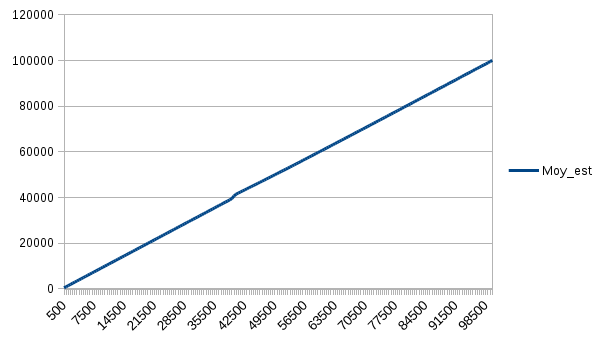
\includegraphics[scale=0.4]{./moy.png}
   \caption{\label{figmoy}Estimate average}
  
\end{figure}

\begin{block}{Bench case}
1000 times the algorithm on random
data of cardinality from 500 to 100000.
\end{block}

\end{frame}

\begin{frame}{Benchmarking}
\begin{figure}[h!]
   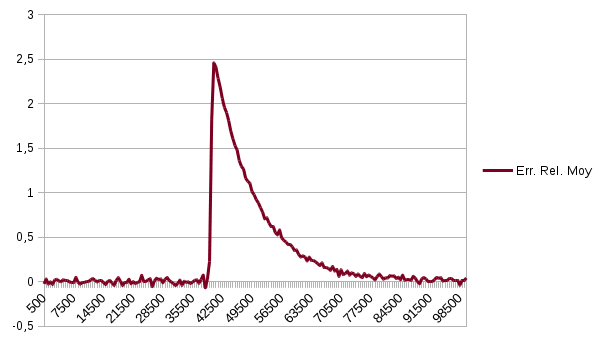
\includegraphics[scale=0.5]{./moy2.png}
   \caption{\label{figerr}Relative error average in percent}
\end{figure}
\end{frame}

\begin{frame}{Benchmarking}
\begin{figure}[h!]
   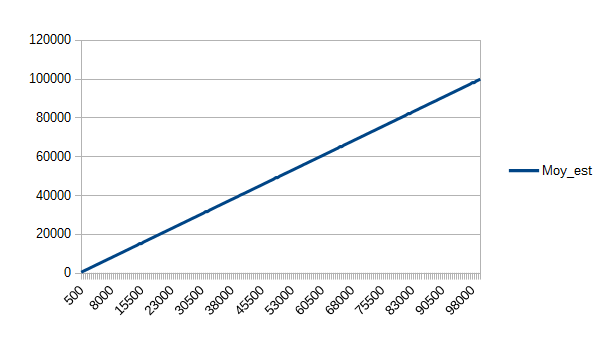
\includegraphics[scale=0.5]{./moy_corr.png}
   \caption{\label{figerr}Corrected error average}
\end{figure}
\end{frame}


\begin{frame}{Benchmarking}
\begin{figure}[h!]
   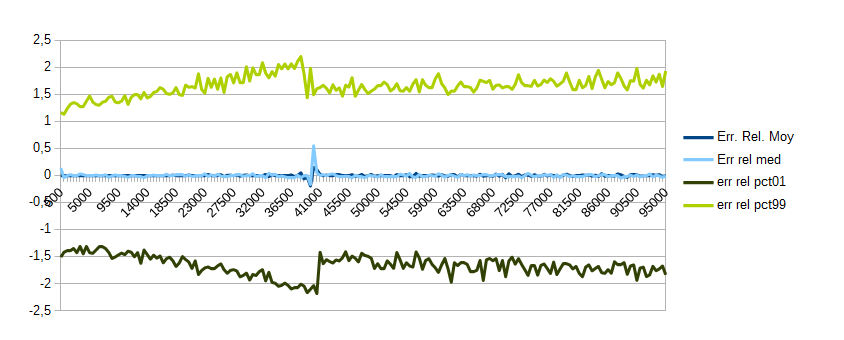
\includegraphics[scale=0.5]{./data_corr.png}
   \caption{\label{figerr}Corrected error average}
\end{figure}
\end{frame}


\begin{frame}{Benchmarking}
\begin{figure}[h!]
   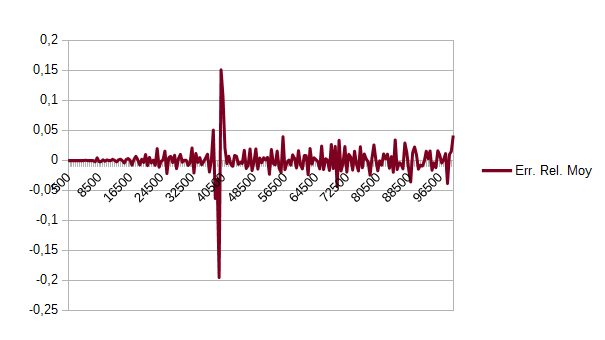
\includegraphics[scale=0.5]{./moy_err.png}
   \caption{\label{figerr} Corrected error average}
\end{figure}
\end{frame}


\begin{frame}{Conclusion}

\begin{block}{Overview of our implementation}
  We implemented the algorithm, but it's not fully optimized. 
\end{block}
  
\begin{block}{Conclusive reflexion}
  Ocaml is too high level to express fine grained memory management
  but it was a funny challenge.
\end{block}

\end{frame}




\end{document}



(*
% rubber: setlist arguments --shell-escape --enable-write18
Local Variables:
compile-command: "rubber -d talk.tex"
ispell-local-dictionary: "francais"
End:
*)



